\documentclass[11pt]{article}
\usepackage[a4paper,margin=1in]{geometry}
\usepackage{amsmath,amssymb,booktabs,graphicx,hyperref,array}
\newcolumntype{L}[1]{>{\raggedright\arraybackslash}p{#1}}
\newcommand{\dd}{\mathrm{d}}
\title{TCV-$\Phi$ and the Standard-Model Derivation Program:\\Exact Core, Candidate Phenomenology, and Claim Boundaries}
\author{Cyrille LECROQ}
\date{\today}
\newcommand{\authoraffiliation}{Independent Researcher}

\begin{document}
\maketitle
\begin{center}
\authoraffiliation
\end{center}

\begin{abstract}
We present a staged derivation program for Standard-Model structure in the two-scalar TCV-$\Phi$ framework, using the frozen Stage~3 to Stage~29 exploration package as the traceable source base. The exact internal core supports an exact $U(1)\times SU(2)\times SU(3)$ gauge-product derivation together with an exact representation-side capstone. On top of this core, the current package supports a strengthened guarded theorem-style internal anomaly-dynamics structure with closed-form unique zero, exact isolated minimum, and analytic symmetry-lock recovery, while still stopping short of an unconditional theorem-level anomaly-cancellation derivation. The external matching layer supports a full Standard-Model crossing claim only within an explicitly tested matching window and must therefore remain window-qualified. The same discipline is applied to later outputs: $\Lambda_{\mathrm{TCV}}$ and $m_{\Phi_2}$ are reported as candidate predictions with explicit residual dependence, whereas $\sin^2(\theta_W)=0.375\pm0.050$ is retained only as a high-scale electroweak matching anchor with a conditional upgrade path. We also summarize candidate routes for generation structure and for a high-scale gauge-coupling meeting near $\Lambda_{\mathrm{TCV}}$. The manuscript is organized to distinguish exact derived results, candidate routes, conditional upgrades, and blocked claims explicitly.
\end{abstract}

\section{Introduction}
The aim of this manuscript is narrow and methodological. We do not present a generic narrative about Standard-Model emergence. We present a staged derivation program, frozen at explicit checkpoints, together with the strongest claim boundary currently supported by the code and data package. The relevant source arc is the Stage~3 to Stage~29 exploration workspace, in which exact internal structure, external matching windows, candidate phenomenological routes, and blocked claims were separated deliberately rather than blended into a single undifferentiated story. The target gauge structure is the Standard-Model Yang--Mills product introduced historically through the nonabelian gauge construction of Yang and Mills and through the electroweak and color frameworks of Glashow, Weinberg, Salam, Gross--Wilczek, and Politzer \cite{YangMills1954,Glashow1961,Weinberg1967,Salam1968,GrossWilczek1973,Politzer1973}.

The central reason for this separation is simple. Different layers of the program have different evidential status. The exact gauge-product derivation and the exact representation-side capstone belong to the internal mathematical core. The anomaly-dynamics package is stronger than a numerical hint but weaker than an unconditional theorem. The hard-prediction outputs, the generation routes, and the conditional unification route all depend on additional matching or route-level assumptions and therefore must be described at that level. Treating these layers as interchangeable would produce category errors and make the paper easy to attack.

The paper therefore follows three rules. First, every major claim is tied to a frozen stage output. Second, every route that is not theorem-level is labeled as candidate or conditional. Third, every blocked claim remains blocked in the main text, not only in internal notes. This is not rhetorical caution. It is part of the result: the package is only scientifically usable if its exact core and its non-exact extensions remain visibly separated.

This program also belongs in the broader landscape of attempts to recover Standard-Model structure from deeper mathematical data. The closest comparison point is the noncommutative-geometry line of Connes and collaborators, where the gauge product is recovered from spectral data rather than from the staged mesoscopic microstructure used here \cite{ConnesLott1990,ChamseddineConnes2007}. Paper~X does not claim to supersede that literature. Its narrower claim is that the frozen TCV-$\Phi$ observable program supplies an independent route to an exact gauge package and a controlled representation-side extension with explicit claim boundaries.

Within that discipline, the paper still has a substantial scope. The exact core reaches an exact $U(1)\times SU(2)\times SU(3)$ gauge-product package together with an exact representation-side capstone and a guarded anomaly-dynamics package. On top of that core, the current frozen workspace supports a windowed Standard-Model crossing package, explicit hard-prediction candidates, a candidate generation-structure package, and a candidate gauge-coupling unification route. The manuscript is organized to make that hierarchy explicit rather than implicit.

\begin{figure}[ht]
    \centering
    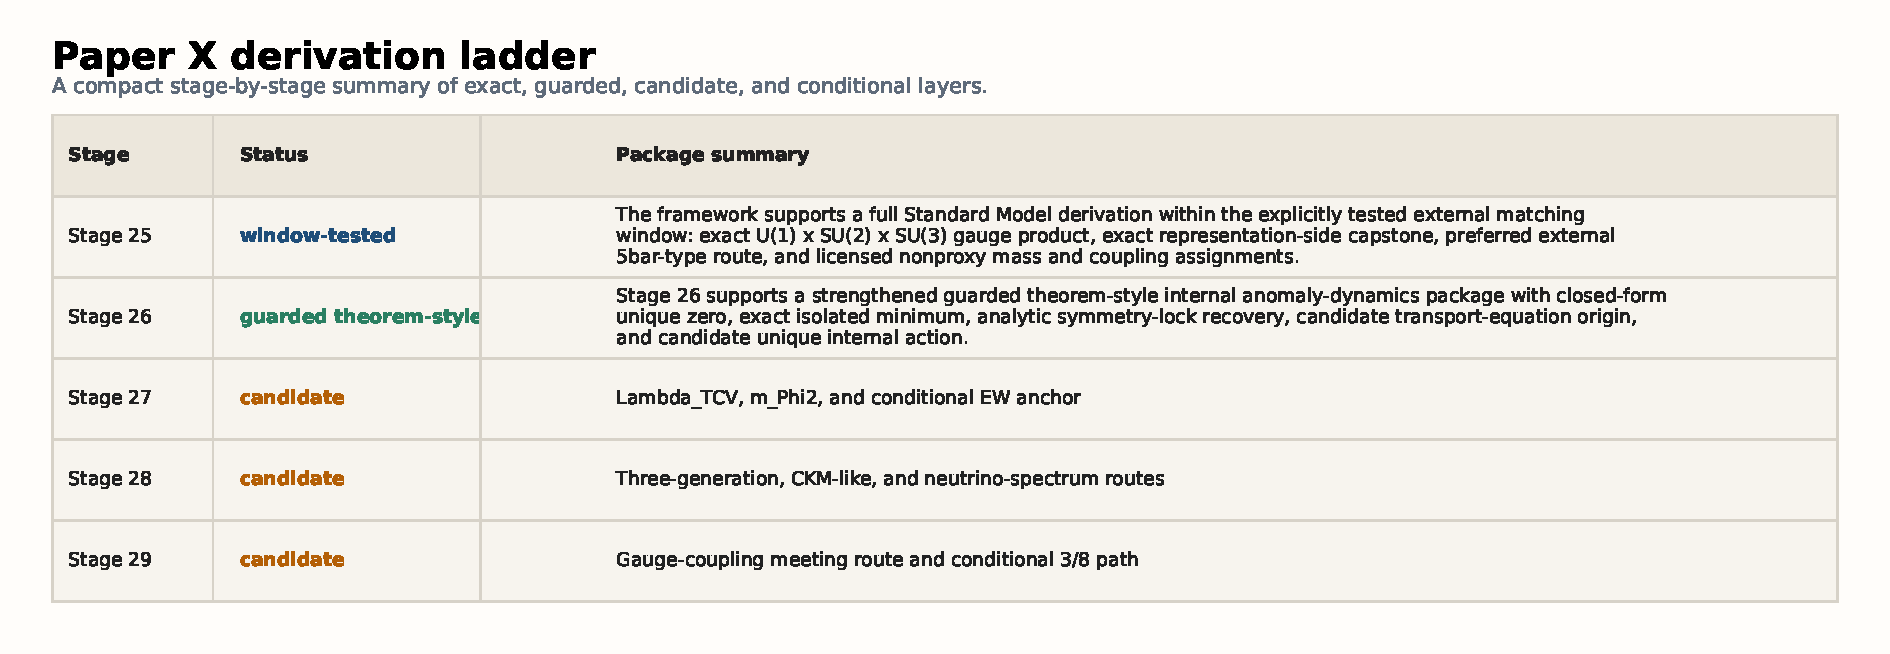
\includegraphics[width=\textwidth]{../figs/fig01-derivation-ladder.pdf}
    \caption{Paper-facing derivation ladder from the Stage~25 windowed crossing package through the Stage~29 conditional route layer. Exact and guarded packages are separated visually from candidate and conditional extensions.}
    \label{fig:derivation-ladder}
\end{figure}

\section{Framework}
The starting point of the program is the minimal TCV-$\Phi$ effective field theory: Einstein gravity coupled to two real scalar degrees of freedom, a heavy structural mode $\Phi_1$ and a light coherent mode $\Phi_2$. In the notation of the earlier TCV-$\Phi$ papers, the physically relevant localized sectors built from these fields are referred to as CC-$\Phi_1$ and CC-$\Phi_2$ \cite{TCVPhiI,TCVPhiII,TCVPhiIX}. For the purposes of the present manuscript, CC-$\Phi_1$ carries the structural vacuum microphysics used throughout the gauge and representation derivation, whereas CC-$\Phi_2$ is retained mainly as part of the parent EFT and as the light bridge re-entering only in the later prediction layer. Concretely, CC-$\Phi_2$ is the ultra-light dark-sector branch of the framework, and its mass scale $m_{\Phi_2}$ appears only in the later prediction layer rather than in the gauge derivation itself.

At the EFT level, the background theory is organized around a two-scalar action of the form
\begin{equation}
S_{\mathrm{TCV}\text{-}\Phi}
=
\int \dd^4x \sqrt{-g}\,
\left[
\frac{1}{2}\left(M_{\mathrm{Pl}}^2+\xi_0 \Phi_1^2\right)R
-\frac{1}{2}(\partial\Phi_1)^2
-\frac{1}{2}(\partial\Phi_2)^2
-V(\Phi_1,\Phi_2)
\right],
\label{eq:tcvphi-action}
\end{equation}
where $\xi_0$ is the non-minimal coupling that sets the high-scale calibration used later in the paper. Equation~\eqref{eq:tcvphi-action} is not yet the Standard-Model derivation. It is the frozen parent EFT from which the microstructural observables, transport diagnostics, and effective algebraic packages are extracted in stages.

The logic of the present manuscript depends on keeping three levels separate. First, there is the parent two-scalar EFT itself, Eq.~\eqref{eq:tcvphi-action}. Second, there is the mesoscopic observable layer built from coherent CC-$\Phi_1$ / CC-$\Phi_2$ structures, transport observables, and reduced slot dictionaries. Third, there is the external matching layer in which some of these reduced structures are compared with Standard-Model packages. The gauge-product and representation results belong primarily to the second level, while the windowed Standard-Model crossing and the later prediction/unification routes belong to the third. This separation is essential: the paper does not claim that Eq.~\eqref{eq:tcvphi-action} alone immediately yields the full Standard Model without the staged observable construction.

In practical terms, the gauge-side derivation uses a frozen five-slot observable basis inherited from the Stage~17 mesoscopic closure and refined through the Stage~25 crossing package. Throughout the paper, the term \emph{frozen basis} refers to the fixed five-slot observable set $\{\mathrm{OBS}_{01},\ldots,\mathrm{OBS}_{05}\}$, which is held constant through all later stages of the program. The negative branch forms a two-slot sector and the positive branch a three-slot sector. The core claim of the paper is that this structured basis supports an exact gauge-product package and an exact representation-side capstone before the later route-level phenomenology is introduced. The framework section is therefore not a review of the whole TCV-$\Phi$ program; it is the minimal statement of the parent EFT and of the staged microstructure-to-observable logic needed to interpret the later sections.

\section{Claim Hierarchy}
The manuscript uses a simple hierarchy throughout: exact internal derivations, supported but window-qualified packages, candidate routes, and blocked claims. Table~\ref{tab:claim-hierarchy} summarizes that hierarchy so that later sections can be read without ambiguity.

\begin{table}[ht]
\centering
\small
\begin{tabular}{p{0.14\linewidth}p{0.62\linewidth}p{0.12\linewidth}}
\toprule
Tier & Claim & Status \\
\midrule
Level A & exact gauge-product derivation & allowed \\
Level A & exact representation-side capstone & allowed \\
Level A & guarded theorem-style internal anomaly-dynamics package & allowed \\
Level B & windowed full-SM crossing package & allowed \\
Level B & candidate hard-prediction package & allowed \\
Level B & candidate generation-structure package & allowed \\
Level B & candidate gauge-coupling unification-route package & allowed \\
Level C & conditional $\sin^2(\theta_W)=3/8$ upgrade route & allowed \\
Level C & CKM-like route & allowed \\
Level C & transport-driven neutrino-spectrum route & allowed \\
Blocked & fully unconditional internal anomaly-cancellation theorem & blocked \\
Blocked & internally derived exact electroweak-angle theorem value & blocked \\
Blocked & licensed gauge-coupling unification claim & blocked \\
Blocked & theorem-level derivation of three generations & blocked \\
Blocked & precision CKM prediction & blocked \\
Blocked & precision neutrino-spectrum prediction & blocked \\
\bottomrule
\end{tabular}
\caption{Claim hierarchy for Paper X. Levels A--C separate derived claims, candidate routes, and conditional upgrades from explicitly blocked claims.}
\label{tab:claim-hierarchy}
\end{table}


In practice, Level~A claims may appear in strong declarative form, Level~B claims remain explicitly window-qualified, and Level~C claims are stated only as routes or conditional upgrades. This matters most for the electroweak angle, gauge-coupling unification, and flavour structure: in the current package, $\sin^2(\theta_W)=3/8$ remains an external matching anchor with a conditional upgrade path, the gauge-coupling meeting remains a candidate route, and the generation/CKM/neutrino structures remain candidate routes rather than theorem-level outputs.

\begin{figure}[ht]
    \centering
    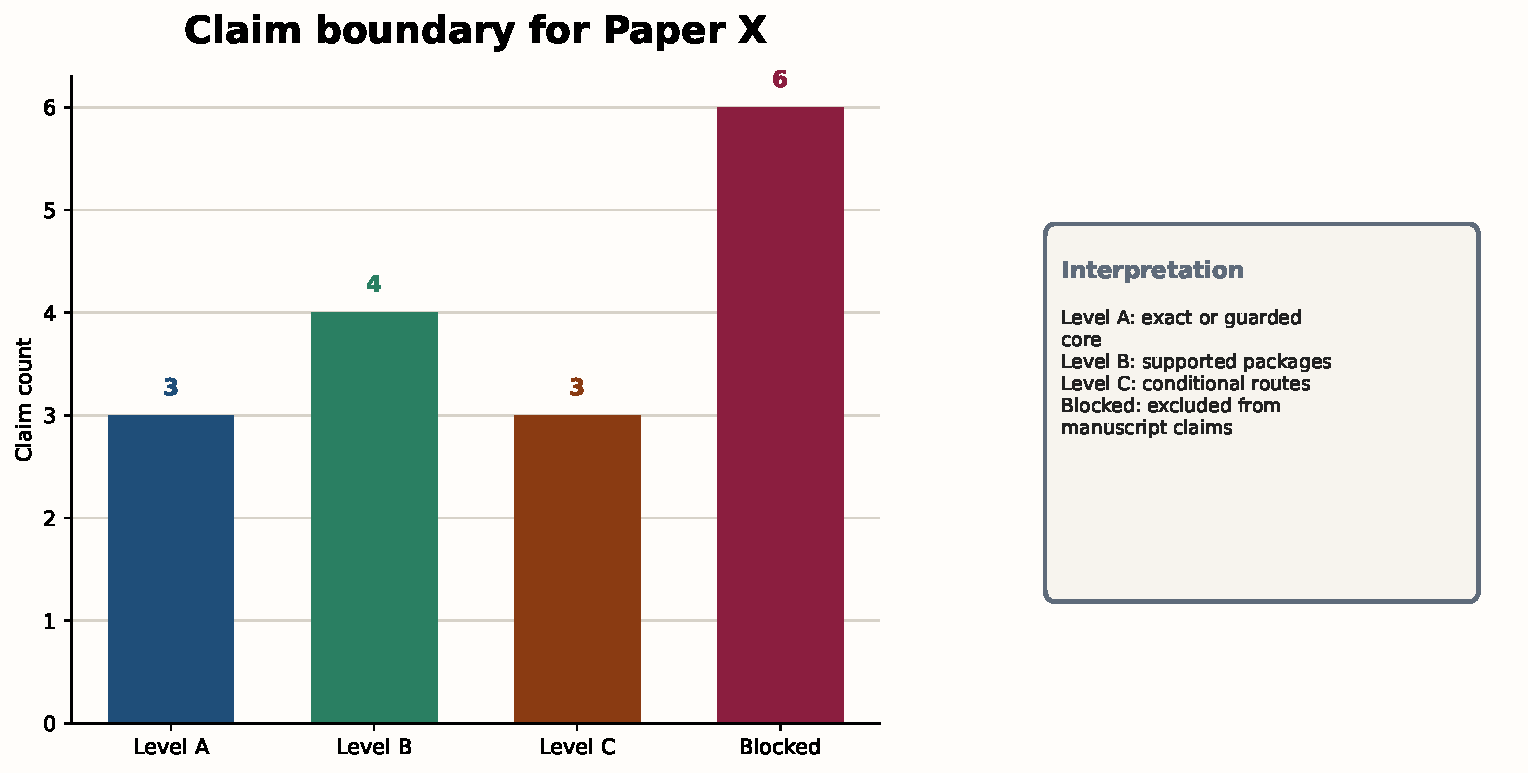
\includegraphics[width=0.82\textwidth]{../figs/fig02-claim-boundary.pdf}
    \caption{Claim hierarchy used throughout Paper~X. Blocked claims remain blocked in the main text and in the visual package.}
    \label{fig:claim-boundary}
\end{figure}

\section{Operational Meaning of ``Exact''}
The term ``exact'' is used in this paper in a restricted operational sense and not as a synonym for a completely unconditional theorem. In the present manuscript, an object is called exact when the staged TCV-$\Phi$ construction closes on a uniquely identified algebraic or representation-level structure with numerically negligible residual ambiguity on the frozen basis and with all tested competing packages excluded at the same stage. This is the sense in which the gauge-product and representation-side statements are exact.

More precisely, ``exact'' in the paper means three things simultaneously. First, the target structure is discrete rather than continuously fit: for example, the relevant output is the gauge-product package $U(1)\times SU(2)\times SU(3)$ rather than a floating deformation parameter. Second, the frozen scans and closure tests identify a single admissible package, or a single admissible point, within the staged observable basis. Third, residual mismatches are treated as numerically negligible at the level of the tested algebraic object, so that no rival package survives at comparable quality. In this sense, exactness here is a closure statement on a specified observable space, not a claim that every surrounding phenomenological layer has already been derived without qualification.

This operational definition is necessary because the paper deliberately combines exact-core statements with route-level extensions. The Stage~15 to Stage~22 arc supports an exact gauge-product plus exact representation-side capstone before external matching is invoked. By contrast, the Stage~25 Standard-Model crossing remains explicitly window-qualified, the Stage~26 anomaly package remains guarded rather than unconditional, and the Stage~27 to Stage~29 outputs remain candidate or conditional. The manuscript therefore uses ``exact'' only for the internal closure layers whose competing alternatives are removed on the frozen basis, and never as shorthand for full phenomenological completeness.

Stated differently, the exact statements in Paper~X are exact relative to the staged observable construction and to the tested discrete competitor space, whereas the later phenomenological statements carry explicit route or window qualifiers. This distinction is not cosmetic. It is the only way to keep the main result both strong and technically honest: exact gauge and representation closure can be defended on its own terms, while the anomaly, flavour, and unification layers remain described at their actual support level.

\section{Tested External Matching Window}
The phrase ``within the tested external matching window'' has a specific operational meaning in this paper. It does not refer to an unspecified tolerance cloud. It refers to the finite conjunction of external route choices and anchor selections under which the Stage~25 crossing package is licensed. In the frozen package, the tested window is centered on the preferred external $\bar{\mathbf{5}}$-type route
\begin{equation}
Y_d=-\frac{1}{2},
\qquad
Y_t=\frac{1}{3},
\label{eq:window-hypercharge-route}
\end{equation}
together with the type-level assignment
\begin{equation}
\mathrm{OBS}_{01}\mapsto \nu_L\text{-like},\quad
\mathrm{OBS}_{02}\mapsto e_L\text{-like},\quad
\mathrm{OBS}_{03,04,05}\mapsto \bar d_R\text{-color-like}.
\label{eq:window-type-map}
\end{equation}
Equations~\eqref{eq:window-hypercharge-route} and~\eqref{eq:window-type-map} define the representation-side entrance into the external matching layer.

The same tested window also contains a specific nonproxy mass-side anchor and a specific nonproxy coupling-side anchor. On the mass side, the preferred frozen anchor is the \texttt{muon\_strange\_anchor} with $L^1$ distance $0.140578\ldots$ to the proxy pattern. On the coupling side, the best anchor retained by the Stage~24 assessment is the \texttt{electroweak\_like} anchor with $L^1$ distance $0.271034\ldots$, together with the preferred mixed electroweak/strong candidate family selected at the disambiguation stage. The Stage~25 crossing claim is therefore licensed only after the route in Eqs.~\eqref{eq:window-hypercharge-route}--\eqref{eq:window-type-map} is combined with those mass and coupling anchor choices.

This definition matters because the window qualifier is not rhetorical. The paper does not claim that every nearby external assignment works equally well, nor that the Standard-Model crossing has already been established in a window-independent sense. The exact gauge-product and representation-side capstone belong to the internal core; the full Standard-Model crossing belongs to the internal core plus the tested external window just described. In practice, the window contains (i) the preferred $\bar{\mathbf{5}}$-type route, (ii) the preferred nonproxy mass anchor, and (iii) the preferred nonproxy coupling anchor/candidate family. Outside that explicitly stated package, the paper returns to candidate-route language rather than licensed crossing language.

\section{Exact SU(3) Core}
The first exact gauge-side result needed in the manuscript is the positive-branch $SU(3)$ package. At the internal rank-2 stage, the reconstructed positive-triplet carrier is summarized by the two Cartan-like directions
\begin{equation}
H_1^{\mathrm{int}}
=
\left(
\frac{1}{2},
-\frac{1}{2},
0
\right),
\qquad
H_2^{\mathrm{emp}}
=
\left(
\frac{1}{2\sqrt{3}},
\frac{1}{2\sqrt{3}},
-\frac{1}{\sqrt{3}}
\right),
\label{eq:su3-cartan-pair}
\end{equation}
written here in the ordered positive-triplet basis $(\mathrm{OBS}_{03},\mathrm{OBS}_{04},\mathrm{OBS}_{05})$. The key internal result of Stage~13 is that the second direction is not inserted independently: it is recovered from the first direction and the $A_2$ rank-2 constraints, with machine-level residual
\begin{equation}
\|H_2^{\mathrm{emp}}-H_2^{\mathrm{der}}\|_\infty
=
3.885780586188048\times 10^{-15}.
\label{eq:su3-h2-residual}
\end{equation}

The corresponding candidate Cartan matrix is
\begin{equation}
C_{\mathrm{int}}
=
\begin{pmatrix}
2.0 & -1.0000000000000138\\
-0.9999999999999858 & 2.0
\end{pmatrix},
\label{eq:su3-cartan-candidate}
\end{equation}
which is compared against the canonical $A_2$ Cartan matrix
\begin{equation}
C_{A_2}
=
\begin{pmatrix}
2 & -1\\
-1 & 2
\end{pmatrix}.
\label{eq:su3-cartan-a2}
\end{equation}
The induced Cartan residual is
\begin{equation}
\|C_{\mathrm{int}}-C_{A_2}\|_\infty
=
1.4210854715202004\times 10^{-14}.
\label{eq:su3-cartan-residual}
\end{equation}

This residual alone is not the full claim. The decisive step is the discrete rank-2 classification test. In the frozen Stage~13 package, the distances from the reconstructed Cartan carrier to the rank-2 Cartan--Killing candidates are
\begin{align}
d(A_2) &= 1.4210854715202004\times 10^{-14},\\
d(B_2) &= 1.0000000000000142,\\
d(G_2) &= 2.000000000000014.
\label{eq:su3-rank2-distances}
\end{align}
so the nearest alternative beyond $A_2$ is order one away. The resulting separation ratio is
\begin{equation}
\frac{d(B_2)}{d(A_2)}
=
70368744177665.0
\simeq
7\times 10^{13}.
\label{eq:su3-separation-ratio}
\end{equation}
This number is one of the central anti-coincidence metrics of the paper: the internal object is not merely numerically close to $A_2$; it is uniquely close to $A_2$ within the discrete rank-2 Cartan list.

The paper therefore uses the following operational proposition.

\paragraph{Proposition 1 (Exact positive-branch $SU(3)$ package).}
Let the positive branch be represented by the internal Cartan pair in Eq.~\eqref{eq:su3-cartan-pair}. If the reconstructed Cartan carrier satisfies the machine-level residuals in Eqs.~\eqref{eq:su3-h2-residual} and \eqref{eq:su3-cartan-residual}, and if the discrete rank-2 Cartan distances satisfy Eq.~\eqref{eq:su3-rank2-distances} with separation ratio \eqref{eq:su3-separation-ratio}, then the positive-branch carrier is uniquely classified as $A_2$ on the frozen basis. In the operational sense defined earlier, this licenses the exact $SU(3)$ gauge-side claim for the positive branch.

The important boundary is that this proposition is an exact internal classification statement, not yet a full Standard-Model statement by itself. It gives the exact $SU(3)$ factor because the internal rank-2 object closes uniquely on $A_2$ with machine-level residuals and with no competing rank-2 Cartan package surviving at comparable distance. The later representation and crossing layers build on this result; they do not replace it.


\section{Exact SU(2) Core}
The negative branch closes on a rank-1 package before the full gauge product is assembled. On the frozen two-slot basis $(D_-,D_+)$, the exact normalized doublet basis is
\begin{equation}
D_-=-\frac{1}{2},\qquad D_+=+\frac{1}{2},
\label{eq:su2-doublet-basis}
\end{equation}
with centered sum and exact unit span,
\begin{equation}
D_-+D_+=0,\qquad D_+-D_-=1.
\label{eq:su2-center-span}
\end{equation}
The raw pair-step observable is first measured internally and then normalized onto the exact half-step basis,
\begin{equation}
\Delta_{\mathrm{pair}}=0.38551710611172874,\qquad
\Delta_{1/2}=\frac{\Delta_{\mathrm{pair}}}{2}=0.19275855305586437,
\label{eq:su2-raw-half-step}
\end{equation}
so that the exact rank-1 carrier is represented as
\begin{equation}
H(D_-)=-\frac{1}{2},\qquad H(D_+)=+\frac{1}{2},\qquad E_+\text{-span}=1,\qquad E_-\text{-span}=-1.
\label{eq:su2-cartan-package}
\end{equation}
At this point the internal rank-1 package satisfies three exact closure identities,
\begin{equation}
\left(\frac{1}{2}+\frac{1}{2}\right)-1=0,
\label{eq:su2-r1}
\end{equation}
\begin{equation}
1+(-1)=0,
\label{eq:su2-r2}
\end{equation}
\begin{equation}
H(D_-)+H(D_+)=0.
\label{eq:su2-r3}
\end{equation}
Equations~\eqref{eq:su2-r1}--\eqref{eq:su2-r3} encode, respectively, exact half-step closure, exact antisymmetric ladder span, and exact trace-like cancellation on the negative branch.

The resulting rank-1 Cartan invariant is then
\begin{equation}
A^{\mathrm{cand}}_{(1)}=2.0,
\label{eq:su2-cartan-invariant}
\end{equation}
which coincides exactly with the unique simple rank-1 Cartan type $A_1$, with nearest-type distance
\begin{equation}
d(A_1)=0.
\label{eq:su2-a1-distance}
\end{equation}
This is the rank-1 analogue of the discrete $A_2$ classification used above for the positive branch: the negative branch does not merely resemble a doublet package qualitatively; it closes exactly on the unique simple rank-1 Cartan object.

The paper therefore uses the following operational proposition.

\paragraph{Proposition 2 (Exact negative-branch $SU(2)$ package).}
Let the negative branch be represented by the normalized doublet basis in Eq.~\eqref{eq:su2-doublet-basis} and by the Cartan/ladder carrier in Eq.~\eqref{eq:su2-cartan-package}. If the exact closure identities \eqref{eq:su2-r1}--\eqref{eq:su2-r3} hold and if the rank-1 Cartan invariant satisfies Eqs.~\eqref{eq:su2-cartan-invariant} and \eqref{eq:su2-a1-distance}, then the negative-branch carrier is uniquely classified as $A_1$ on the frozen basis. In the operational sense defined earlier, this licenses the exact $SU(2)$ gauge-side claim for the negative branch.

As with the $SU(3)$ branch, this statement is internal and classificatory: it is not yet a full electroweak or Standard-Model claim in isolation. Its role is narrower and more precise. It identifies an exact rank-1 factor with zero classification distance and with no competing simple rank-1 type surviving on the frozen doublet basis. The later gauge-product and representation stages depend on this exact $A_1$ closure.


\section{Exact \texorpdfstring{$U(1)$}{U(1)} Core}
The abelian factor is not recovered from a nonabelian Cartan classification. It is recovered as the unique surviving scalar sign axis carried by the frozen five-slot observable package. On the ordered basis $(\mathrm{OBS}_{01},\mathrm{OBS}_{02},\mathrm{OBS}_{03},\mathrm{OBS}_{04},\mathrm{OBS}_{05})$, the exact charge axis is
\begin{equation}
Q_{U(1)} = (-1,-1,+1,+1,+1).
\label{eq:u1-charge-axis}
\end{equation}
This axis coincides with the polarity split inherited from the precursor grammar,
\begin{equation}
\{\mathrm{OBS}_{01},\mathrm{OBS}_{02}\}\in Q_{-},
\qquad
\{\mathrm{OBS}_{03},\mathrm{OBS}_{04},\mathrm{OBS}_{05}\}\in Q_{+},
\label{eq:u1-sector-split}
\end{equation}
and therefore defines a unique negative/positive scalar direction that survives the later nonabelian branch refinements.

The exact abelian generator is then the scalar action induced by this sign axis,
\begin{equation}
T_{U(1)}\,|\mathrm{OBS}_i\rangle = q_i|\mathrm{OBS}_i\rangle,
\qquad
(q_1,q_2,q_3,q_4,q_5)=(-1,-1,+1,+1,+1).
\label{eq:u1-generator-action}
\end{equation}
Because the carrier is one-dimensional in the algebraic sense, the commutator closes identically,
\begin{equation}
[T_{U(1)},T_{U(1)}]=0,
\qquad
\|[T_{U(1)},T_{U(1)}]\|=0.
\label{eq:u1-zero-commutator}
\end{equation}
The abelian licensing step is therefore not a proximity argument but a uniqueness argument: no second independent scalar sign axis survives on the frozen basis once the joint sign split and branch decomposition are fixed.

A useful boundary must be stated explicitly here. The exact abelian object in Eqs.~\eqref{eq:u1-charge-axis}--\eqref{eq:u1-zero-commutator} is the internal $U(1)$ carrier. It is not yet the externally normalized hypercharge assignment used later in the Stage~23 $\bar{\mathbf 5}$-type matching route. The later normalized values
\begin{equation}
Y_d=-\frac{1}{2},\qquad Y_t=+\frac{1}{3}
\label{eq:u1-later-hypercharge-boundary}
\end{equation}
belong to the external matching layer. They refine the exact sign axis for phenomenological identification; they do not replace the internal abelian generator.

The paper therefore uses the following operational proposition.

\paragraph{Proposition 3 (Exact scalar-axis $U(1)$ package).}
Let the frozen five-slot basis carry the scalar sign axis in Eq.~\eqref{eq:u1-charge-axis}. If this axis remains the unique surviving scalar direction under the sector split \eqref{eq:u1-sector-split}, and if the induced generator action satisfies Eq.~\eqref{eq:u1-generator-action} with identically vanishing commutator residual \eqref{eq:u1-zero-commutator}, then the frozen basis supports an exact abelian $U(1)$ factor in the operational sense defined earlier.

This proposition is the abelian complement to Propositions~1 and~2. The $U(1)$ factor is exact because its scalar carrier is unique and because its algebra closes with zero commutator residual by construction. What remains for later stages is not the existence of the abelian factor itself, but its phenomenological normalization and its role inside the exact direct product $U(1)\times SU(2)\times SU(3)$.


\section{Preferred External \texorpdfstring{$\bar{\mathbf 5}$}{5bar}-Type Route}
The most important representation-side result above the pure gauge core is the preferred external five-slot route identified in Stage~23. This result must be stated explicitly because it is the bridge between the exact internal dictionary and the later windowed Standard-Model crossing. The bridge is not a theorem-level flavour statement, but it is stronger than an unconstrained phenomenological guess.

The starting point is the distinction between the exact internal abelian sign carrier and the later external normalization used for physical-type matching. If the negative doublet slots are assigned a common external normalization $Y_d$ and the positive triplet slots are assigned a common external normalization $Y_t$, then the five-slot neutrality condition reads
\begin{equation}
2Y_d + 3Y_t = 0.
\label{eq:fivebar-neutrality}
\end{equation}
Within the tested Stage~23 hypothesis family, the raw uniform choice
\begin{equation}
Y_d=-1,\qquad Y_t=+1
\label{eq:fivebar-raw-choice}
\end{equation}
is excluded because it gives
\begin{equation}
2Y_d+3Y_t = 1 \neq 0,
\label{eq:fivebar-raw-exclusion}
\end{equation}
and therefore fails the five-slot gravitational neutrality test. The preferred normalized route is instead
\begin{equation}
Y_d=-\frac{1}{2},\qquad Y_t=+\frac{1}{3},
\label{eq:fivebar-preferred-normalization}
\end{equation}
for which
\begin{equation}
2Y_d+3Y_t = 0.
\label{eq:fivebar-preferred-neutrality}
\end{equation}
Using the exact doublet $T_3$ assignments from the negative branch,
\begin{equation}
T_3(\mathrm{OBS}_{01})=+\frac{1}{2},\qquad T_3(\mathrm{OBS}_{02})=-\frac{1}{2},
\qquad T_3(\mathrm{OBS}_{03,04,05})=0,
\label{eq:fivebar-t3-assignments}
\end{equation}
the charge assignments induced by $Q=T_3+Y$ are
\begin{equation}
Q(\mathrm{OBS}_{01})=0,
\qquad
Q(\mathrm{OBS}_{02})=-1,
\qquad
Q(\mathrm{OBS}_{03,04,05})=+\frac{1}{3}.
\label{eq:fivebar-charge-assignments}
\end{equation}
All three triplet slots therefore carry the same electric charge $+1/3$, which is the expected charge degeneracy under color rotation and serves as a non-trivial self-consistency check of the \texorpdfstring{$\bar{\mathbf 5}$}{5bar} assignment. This is precisely the type-level pattern selected in the frozen Stage~23 assessment,
\begin{equation}
\mathrm{OBS}_{01}\mapsto \nu_L\text{-like},
\quad
\mathrm{OBS}_{02}\mapsto e_L\text{-like},
\quad
\mathrm{OBS}_{03,04,05}\mapsto \bar d_R\text{-color-like}.
\label{eq:fivebar-type-map}
\end{equation}
Within the tested hypothesis family, $(Y_d,Y_t)=(-1/2,+1/3)$ is the unique neutral solution admitting standard charge quantization simultaneously on the doublet and triplet branches. The tested integer competitor,
\begin{equation}
Y_d=-\frac{3}{2},\qquad Y_t=+1,
\label{eq:fivebar-integer-competitor}
\end{equation}
is still neutral under Eq.~\eqref{eq:fivebar-neutrality}, but it fails the type-pattern test because it produces an integer-charged triplet and a non-leptonic doublet rather than the pattern in Eqs.~\eqref{eq:fivebar-charge-assignments}--\eqref{eq:fivebar-type-map}.

The paper therefore uses the following operational proposition.

\paragraph{Proposition 4 (Preferred external \texorpdfstring{$\bar{\mathbf 5}$}{5bar} route).}
Consider the five-slot package equipped with the exact internal gauge factors from Propositions~1--3 and with the external two-parameter normalization $(Y_d,Y_t)$. If the five-slot neutrality condition \eqref{eq:fivebar-neutrality} is imposed, if the charge operator is evaluated through $Q=T_3+Y$ using the exact negative-branch $T_3$ values in Eq.~\eqref{eq:fivebar-t3-assignments}, and if the admissible route is additionally required to realize the leptonic-doublet / down-type-color-triplet pattern in Eq.~\eqref{eq:fivebar-type-map}, then the preferred tested route is the normalized assignment in Eq.~\eqref{eq:fivebar-preferred-normalization}. In the operational sense used in this paper, this licenses a preferred external \texorpdfstring{$\bar{\mathbf 5}$}{5bar} matching route on the tested window.

This proposition is intentionally narrower than a full $SU(5)$ matter theorem. It does not say that the complete $SU(5)$ matter content has been derived, and it does not say that exact physical flavour names are already licensed independently of the tested window. What it says is more precise: once the exact internal gauge package is fixed, the tested external normalization and type-pattern filters select a unique preferred five-slot route of $\bar{\mathbf 5}$ type. This is the representation-side bridge used later in the Stage~25 windowed Standard-Model crossing, and it is one of the central results of the paper, with its claim boundary kept explicit.

\section{Gauge Product Assembly}
Propositions~1--3 supply the exact gauge-side factors $SU(3)$, $SU(2)$, and $U(1)$ on the frozen basis, while Proposition~4 supplies the preferred external \texorpdfstring{$\bar{\mathbf 5}$}{5bar}-type route that bridges this gauge core to the later windowed Standard-Model crossing. The remaining gauge-side step is to show that these three exact factors assemble as a direct product rather than merely coexist as separate algebras.

\begin{table}[ht]
\centering
\footnotesize
\setlength{\tabcolsep}{4pt}
\begin{tabular}{L{0.09\linewidth}L{0.18\linewidth}L{0.50\linewidth}L{0.13\linewidth}}
\toprule
Stage & Package & Claim-safe summary & Status \\
\midrule
25 & Windowed SM crossing & Exact $U(1)\times SU(2)\times SU(3)$ gauge product, exact representation-side capstone, preferred external $\bar{\mathbf{5}}$-type route, and licensed nonproxy mass/coupling assignments in the tested external window. & window-tested \\
26 & Anomaly dynamics & Strengthened guarded theorem-style internal anomaly-dynamics package with closed-form unique zero, exact isolated minimum, analytic symmetry-lock recovery, candidate transport-equation origin, and candidate unique internal action. & guarded \\
27 & Hard predictions & Candidate package for $\Lambda_{\mathrm{TCV}}$, $m_{\Phi_2}$, and a conditional electroweak anchor. & candidate \\
28 & Generation routes & Candidate three-generation, CKM-like, and transport-driven neutrino-spectrum routes. & candidate \\
29 & Unification route & Candidate gauge-coupling meeting route near $\Lambda_{\mathrm{TCV}}$ and conditional $3/8$ path. & candidate \\
\bottomrule
\end{tabular}
\caption{Stage-wise summary of the Stage~25--29 pre-paper package.}
\label{tab:result-summary}
\end{table}


The product assembly is exact because the supports are sector-separated and the abelian carrier acts uniformly inside each sector. On the frozen basis, the nonabelian supports satisfy
\begin{equation}
\mathrm{supp}(SU(2)) = \{\mathrm{OBS}_{01},\mathrm{OBS}_{02}\},
\qquad
\mathrm{supp}(SU(3)) = \{\mathrm{OBS}_{03},\mathrm{OBS}_{04},\mathrm{OBS}_{05}\},
\label{eq:gauge-supports}
\end{equation}
so that the cross-sector commutator vanishes by disjoint support,
\begin{equation}
[G_{SU(3)},G_{SU(2)}]=0,
\qquad
\|[G_{SU(3)},G_{SU(2)}]\|=0.
\label{eq:gauge-cross-sector-zero}
\end{equation}
For the abelian factor, the internal $U(1)$ carrier is scalar and uniform on each sector,
\begin{equation}
T_{U(1)}|_{Q_-}=-I_2,
\qquad
T_{U(1)}|_{Q_+}=+I_3,
\label{eq:gauge-u1-sector-identity}
\end{equation}
which implies
\begin{equation}
[T_{U(1)},G_{SU(2)}]=0,
\qquad
[T_{U(1)},G_{SU(3)}]=0,
\label{eq:gauge-u1-commutators-zero}
\end{equation}
because $[cI,G]=0$ identically on each sector.

\paragraph{Proposition 5 (Exact gauge direct product).}
Let the frozen basis carry the exact $SU(3)$, $SU(2)$, and $U(1)$ factors from Propositions~1--3. If the sector supports satisfy Eq.~\eqref{eq:gauge-supports}, if the nonabelian cross-sector commutator vanishes as in Eq.~\eqref{eq:gauge-cross-sector-zero}, and if the abelian generator is sectorwise scalar as in Eq.~\eqref{eq:gauge-u1-sector-identity}, so that the mixed commutators vanish as in Eq.~\eqref{eq:gauge-u1-commutators-zero}, then the exact gauge algebra on the frozen basis is
\begin{equation}
\mathfrak g_{\mathrm{int}} = \mathfrak u(1) \oplus \mathfrak{su}(2) \oplus \mathfrak{su}(3).
\label{eq:exact-gauge-product}
\end{equation}
In the operational sense of this paper, this licenses the exact direct-product gauge claim.

This assembly statement is the point at which the separate gauge factors become a single exact internal core. The first layer is exact and internal: discrete Cartan classification on the positive branch, exact rank-1 closure on the negative branch, a unique scalar-axis abelian carrier, and exact cross-factor commutativity. The second layer is exact only up to the tested external window: the preferred \texorpdfstring{$\bar{\mathbf 5}$}{5bar}-type normalization and the Stage~25 crossing package. This distinction is essential because the paper claims a true exact gauge product, but only a window-qualified Standard-Model crossing.

Stage~26 then hardens the same backbone by isolating the anomaly-dynamics structure. The package contains a closed-form unique zero, an exact isolated minimum, analytic symmetry-lock recovery, and a candidate transport/action interpretation. This is materially stronger than a fit or heuristic stability argument, but it still stops short of a fully unconditional theorem-level anomaly-cancellation derivation. That blocked endpoint must remain blocked in the manuscript.

Taken together, Stages~25 and~26 define the safe exact-core statement for Paper~X: the program reaches an exact gauge-product derivation, an exact representation-side closure on the tested five-slot package, and a strengthened guarded internal anomaly package. Later phenomenological routes are built on top of this frozen core; they do not retroactively define it.

\section{Anomaly-Dynamics Package}
The anomaly-dynamics package is the point at which the internal derivation ceases to be merely classificatory and acquires a theorem-style dynamical form. Stage~26 is stronger than a numerical selection mechanism because it contains a closed-form zero, an exact isolated minimum, and an analytic lock structure. It is weaker than an unconditional theorem because the final forcing from full internal dynamics to a uniquely licensed anomaly-cancellation theorem is still not established.

The current endpoint is therefore described as a guarded theorem-style internal anomaly-dynamics object. In concrete terms, it contains:
\begin{itemize}
    \item closed-form unique zero;
    \item exact isolated minimum;
    \item analytic symmetry-lock recovery;
    \item candidate transport-equation origin;
    \item candidate unique internal action.
\end{itemize}
Each element does a different job. The closed-form unique zero removes dependence on local scanning for the existence and uniqueness of the preferred anomaly-neutral point. The exact isolated minimum upgrades that point from a merely admissible solution to a uniquely preferred one in the current analytic action. The symmetry-lock package shows that the same point is recovered from exact algebraic locking conditions, rather than from a single numerical objective only. Finally, the transport/action readings show that the package is not completely ad hoc: there is a candidate dynamical interpretation tying the preferred point to internal transport closure and to an exact action-like object.

What the package does not yet provide is equally important. The candidate transport origin is not yet forced uniquely by the full internal dynamics. The candidate internal action is not yet licensed as the unique dynamical action in a theorem-level sense. For that reason, the paper must avoid unconditional language such as ``anomaly cancellation is fully derived from first principles'' or ``the internal anomaly theorem is complete.'' The correct formulation is that the workspace supports a strengthened guarded theorem-style anomaly-dynamics package whose exact zero and exact minimum are analytically controlled, while the final unconditional forcing step remains open.

This distinction matters because the anomaly package is the most delicate part of the internal derivation. Stated at the proper level, it becomes a strength rather than a weakness: the paper shows exactly how far the internal derivation goes, exactly where the remaining theorem gap sits, and exactly why later phenomenological routes must be read as extensions built on a guarded internal core rather than as direct corollaries of a fully closed theorem.

\section{Hard Predictions}
Stage~27 contributes three explicit values with equally explicit claim boundaries.

\begin{table}[ht]
\centering
\footnotesize
\setlength{\tabcolsep}{4pt}
\begin{tabular}{L{0.20\linewidth}L{0.23\linewidth}L{0.22\linewidth}L{0.23\linewidth}}
\toprule
Item & Value & Category & Boundary \\
\midrule
$\Lambda_{\mathrm{TCV}}$ & $\sim 7.7\times 10^{18}\,\mathrm{GeV}$ & candidate calibration & benchmark-dependent \\
$m_{\Phi_2}$ & $1.0\times 10^{-22}\,\mathrm{eV}$ & candidate prediction & anchor-based normalization \\
$\sin^2(\theta_W)$ & $0.375\pm0.050$ & EW matching anchor & not internally derived \\
Generation family & muon/strange anchor & candidate route & not theorem-level \\
CKM-like route & margin $=0.150482$ & candidate route & not precision CKM \\
Neutrino route & 2nd-gen neutrino-like & candidate route & not quantitative spectrum \\
Unification route & target $[0.85,1.15]$ & candidate route & no RG closure \\
\bottomrule
\end{tabular}
\caption{Headline numbers and route-level outputs exported into Paper X.}
\label{tab:prediction-routes}
\end{table}


The hard-prediction package currently contains three different kinds of outputs. First, there is a candidate high scale, $\Lambda_{\mathrm{TCV}}$, tied to the frozen benchmark choice for $\xi_0$. Second, there is a candidate dark-sector mass scale, $m_{\Phi_2}$, sitting in the fuzzy-dark-matter range. Third, there is a high-scale electroweak anchor, expressed as $\sin^2(\theta_W)=0.375\pm0.050$. These three outputs do not have identical epistemic status. The first is a benchmark-sensitive calibration, the second is a candidate prediction with anchor-dependent normalization, and the third is an external matching anchor whose upgrade path remains conditional.

Two points must remain explicit:
\begin{itemize}
    \item $\Lambda_{\mathrm{TCV}}$ and $m_{\Phi_2}$ are candidate outputs with residual benchmark/anchor dependence;
    \item $\sin^2(\theta_W)$ is currently an external matching anchor, not an internally derived electroweak theorem value.
\end{itemize}

The electroweak case deserves especially careful wording. Earlier exploratory layers of the project contain coupling-anchor structures and normalized patterns that can be numerically confused with an electroweak prediction if categories are blurred. The current paper package does not permit that blur. At the present stage, $\sin^2(\theta_W)=3/8$ is not claimed as a derived theorem output from the internal TCV-$\Phi$ dynamics. It is a conservative high-scale matching anchor, with an explicit interval, and with a conditional upgrade path only if the later gauge-coupling meeting route is established. That claim discipline must remain visible both in the prose and in any figure caption or table discussion.

By contrast, $\Lambda_{\mathrm{TCV}}$ and $m_{\Phi_2}$ can be used more directly as candidate predictions, provided their residual dependence is stated rather than hidden. The hard-prediction package therefore consists of a benchmark-sensitive high scale, a dark-sector mass candidate of immediate phenomenological interest, and a conditional electroweak anchor that is informative but not yet internally licensed as derived. This formulation makes the paper physically meaningful while remaining conservative enough to survive methodological scrutiny.

\begin{figure}[ht]
    \centering
    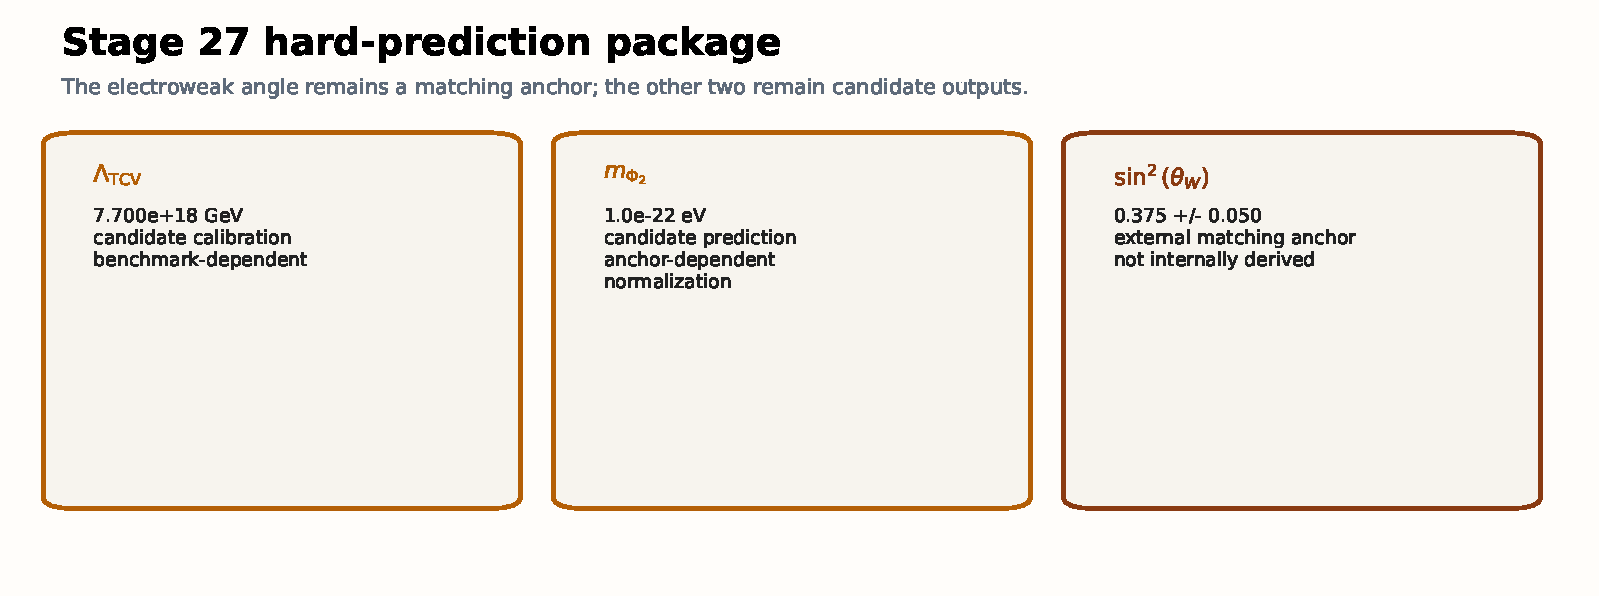
\includegraphics[width=\textwidth]{../figs/fig03-hard-predictions.pdf}
    \caption{Stage~27 paper-facing prediction panel. The electroweak-angle entry is retained explicitly as an external matching anchor rather than an internally derived theorem output.}
    \label{fig:hard-predictions}
\end{figure}

\section{Generation Routes}
Stage~28 contributes a coherent candidate package containing:
\begin{itemize}
    \item a ternary generation route;
    \item a CKM-like small-but-nonzero mixing route;
    \item a transport-driven neutrino-spectrum route.
\end{itemize}
The section therefore uses structural route logic and explicit falsifiability conditions rather than theorem-level flavour language. The correct claim level here is not ``the theory derives flavour'' but rather ``the current frozen package supports a disciplined flavour-side route structure.'' That distinction is crucial. The generation package is one of the most interesting parts of the later-stage program, but it is also one of the easiest places to overclaim if the structural and phenomenological levels are not kept separate.

The first component is the ternary generation route. The argument is not that the number three has already been proven from first principles in a theorem-level sense. The argument is that the frozen package now contains a coherent ternary route: the positive branch is structurally triplet-like, the tested external family space is ternary, and the preferred family assignment is unique within that tested space. This is enough to justify a real generation-origin program and to motivate the discussion of family structure in the paper. It is not enough to state that the existence of exactly three generations has already been derived in a window-independent way.

The second component is the CKM-like route. Here the relevant object is not a fitted matrix but the nonzero triplet imbalance and the fact that it is neither vanishing nor extreme. In the current package, the triplet branch is not democratic and not maximally split. That supports a near-diagonal hierarchical mixing route in which inter-generation mixing is present but remains subordinate to the dominant diagonal organization. This is the safe and useful claim. The unsafe claim would be to identify this route directly with a precision CKM prediction or to imply that the numerical Cabibbo--Kobayashi--Maskawa structure has already been derived.

The third component is the transport-driven neutrino-spectrum route. The key point is that the robust light-pair transport asymmetry lands, under the current assignment package, on the neutrino-like / charged-lepton-like branch rather than on the color triplet branch. This gives a concrete route by which transport asymmetry can be connected to neutrino-sector softness or splitting. Again, the safe statement is structural: the package supports a neutrino-spectrum route. The blocked statement is quantitative: the workspace does not yet provide a licensed prediction for neutrino mass splittings or ordering.

Taken together, these three components give Paper~X a credible flavour-side extension without forcing the paper into a false claim of completed flavour derivation. The resulting route package consists of ternary family structure, small-but-nonzero hierarchical mixing, and transport-sensitive neutrino-sector behavior. Each of these routes is scientifically useful because each comes with an explicit falsification path. None of them closes the flavour problem at theorem level.

\begin{figure}[ht]
    \centering
    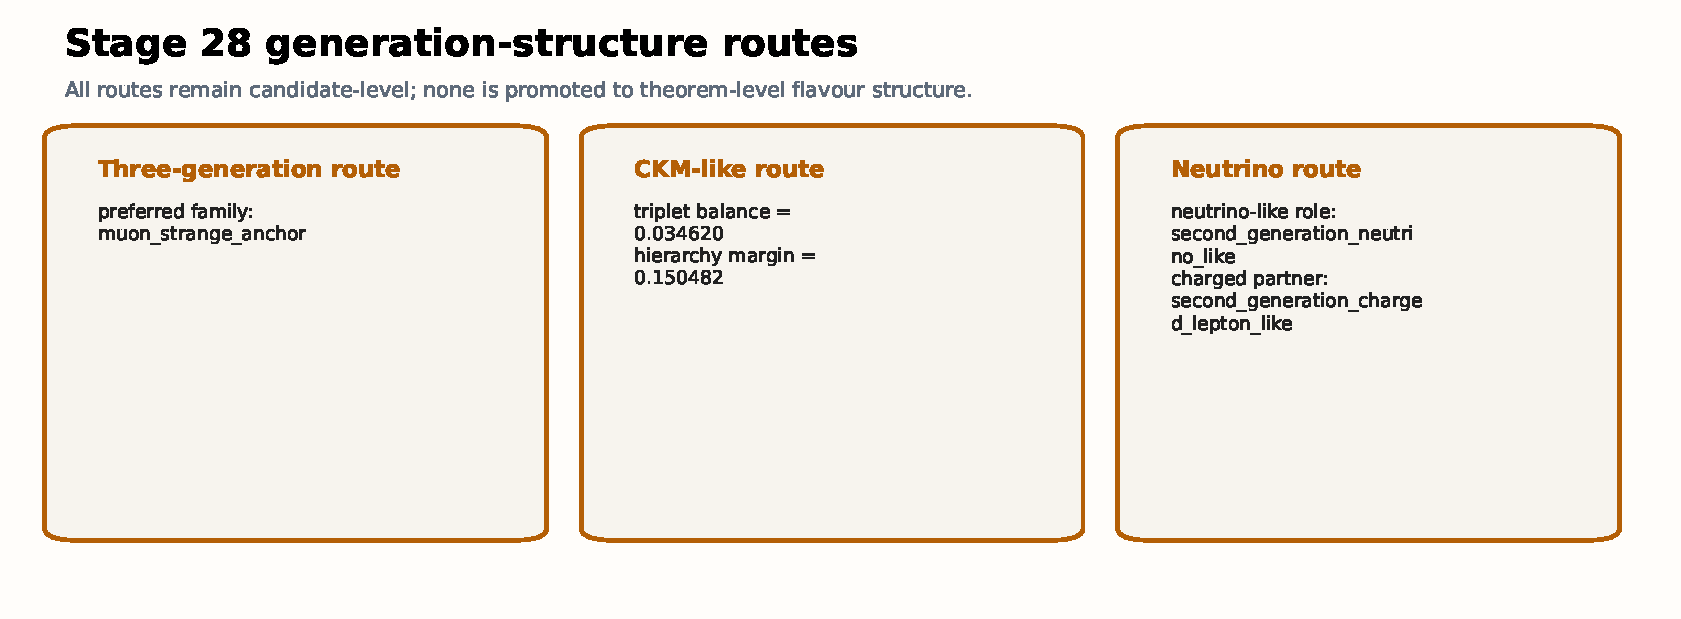
\includegraphics[width=\textwidth]{../figs/fig04-generation-routes.pdf}
    \caption{Stage~28 generation-side route package. These objects are presented as candidate structures rather than theorem-level flavour outputs.}
    \label{fig:generation-routes}
\end{figure}

\section{Conditional Unification Route}
Stage~29 is presented as a candidate route package rather than as a completed GUT derivation. Its current content is:
\begin{itemize}
    \item a structured low-scale mixed family is available;
    \item a candidate high-scale meeting window near $\Lambda_{\mathrm{TCV}}$ is available;
    \item the $3/8$ electroweak value has a conditional upgrade path if a disciplined coupling meeting is established.
\end{itemize}
Neither gauge-coupling unification nor the $3/8$ value is currently licensed as a derived result. This section is where the paper is most exposed to overstatement, because the numerical and representational ingredients can tempt one to read the package as an already completed unification story. The current frozen outputs do not support that stronger reading. What they support is a conditional route from the existing coupling-side package toward a possible high-scale meeting near $\Lambda_{\mathrm{TCV}}$.

The low-scale input to this route is the unique mixed electroweak/strong coupling family selected in the tested external space. The high-scale endpoint is not an already derived renormalization-group trajectory, but an explicit candidate meeting window near $\Lambda_{\mathrm{TCV}}$. Between them, the package supplies a running direction: structured splitting at low scale and flattening toward a high-scale target. This is enough to make the route scientifically meaningful. It is not enough to say that the couplings are now known to unify.

The role of $\sin^2(\theta_W)=3/8$ is framed inside this logic and nowhere else. At the present stage, the value is not an internally derived electroweak theorem output. Instead, it is a conditional electroweak upgrade rule. If a disciplined gauge-coupling meeting can be established near $\Lambda_{\mathrm{TCV}}$, then the current external electroweak anchor can be upgraded from a pure matching anchor to a conditional derivation route. This conditional structure is worth highlighting because it explains why the value remains physically interesting without pretending that the last RG closure step has already been completed.

\begin{figure}[ht]
    \centering
    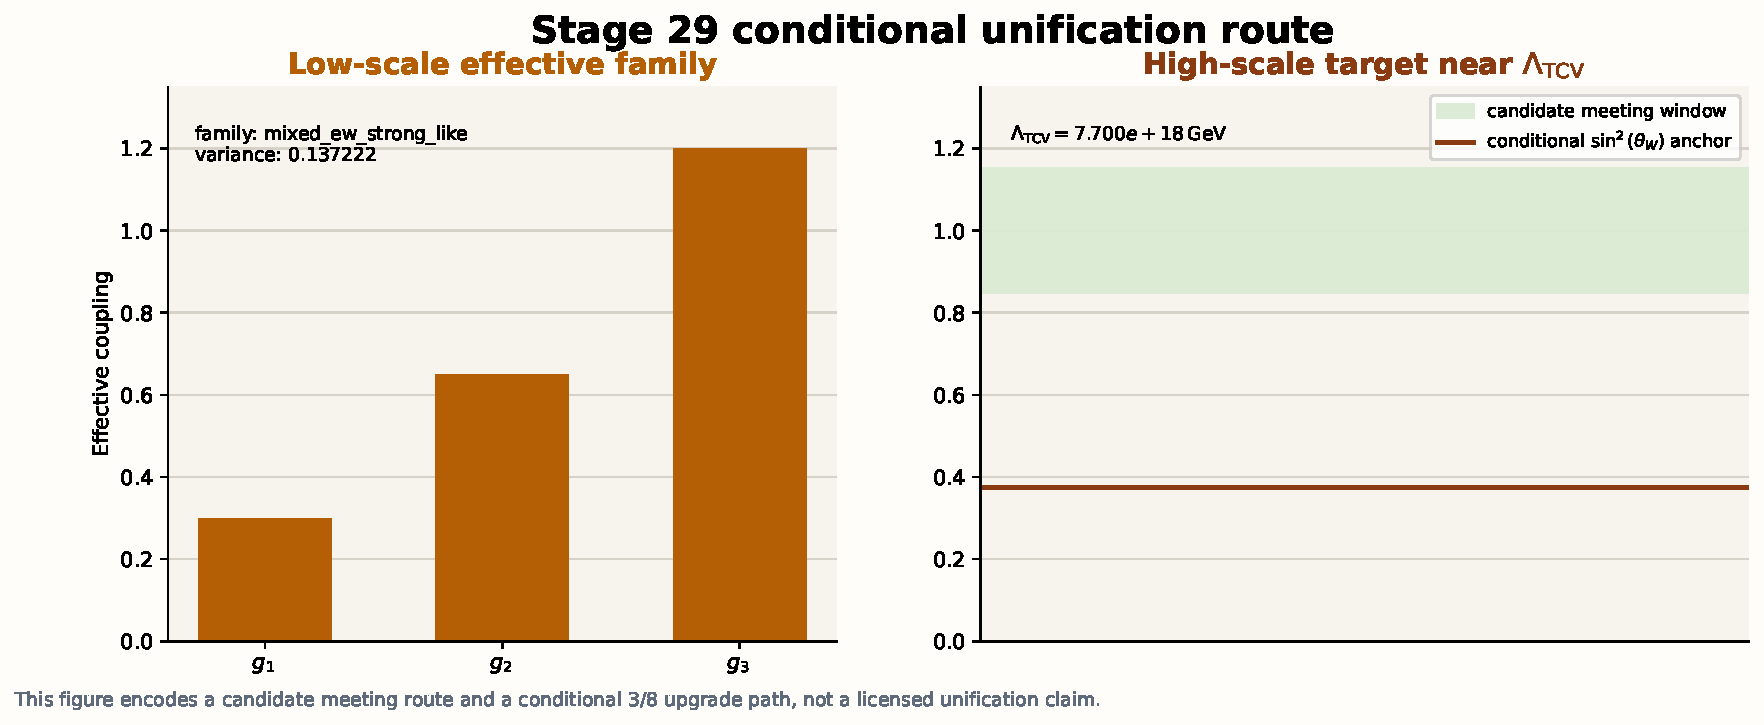
\includegraphics[width=\textwidth]{../figs/fig05-unification-route.pdf}
    \caption{Stage~29 conditional unification route. The figure encodes a candidate high-scale meeting route and a conditional electroweak-angle upgrade path, not a licensed unification claim.}
    \label{fig:unification-route}
\end{figure}

The unification route therefore has a double status. Positively, the project now contains a genuine unification-route package rather than a vague aspiration: there is a low-scale mixed family, a high-scale target window, and a conditional electroweak upgrade path. Negatively, the RG-consistent meeting itself remains unlicensed, and that blocked state remains explicit. This makes the section scientifically sharper because it tells the reader exactly what the package would still need in order to cross from a candidate route to a licensed unification claim.

\section{Claim Boundary and Falsification Map}
This section gathers the falsification maps from the Stage~27, Stage~28, and Stage~29 packages. Its role is to make clear:
\begin{itemize}
    \item what would kill a candidate route;
    \item what would only weaken it;
    \item which statements remain claim-boundary rules rather than phenomenological predictions.
\end{itemize}
The following three subsections track the frozen Stage outputs from which the falsification rules are drawn. This is not a defensive appendix but part of the scientific content of the paper: once a manuscript contains exact core results together with candidate phenomenological routes, the reader must be told not only what is supported, but also what would falsify each supported route and what remains outside the currently licensed claim set.

\subsection{Stage~27 falsifiers}
The Stage~27 falsification map already imposes the first important distinction. $\Lambda_{\mathrm{TCV}}$ and $m_{\Phi_2}$ are candidate outputs that can be weakened or killed by changes in calibration or anchor structure, whereas the electroweak quantity is not yet in the same category. Its current falsification logic applies to an external matching anchor and to its conditional upgrade path, not to an internally derived theorem value. This distinction must remain visible wherever the Stage~27 outputs are summarized.

\subsection{Stage~28 falsifiers}
The Stage~28 falsification map plays a similar role for the flavour-side extensions. The ternary generation route, CKM-like route, and transport-driven neutrino-spectrum route are all scientifically useful because each one can be weakened or falsified without collapsing the exact internal core. This modularity is important. A failed generation route would not erase the exact gauge-product derivation; it would only restrict the paper's flavour-side extension claims. Stating this explicitly makes the paper methodologically stronger, because it shows that the program can lose secondary routes without losing its exact core.

\subsection{Stage~29 falsifiers}
The Stage~29 falsification map performs the same function for the conditional unification narrative. It tells the reader what would count as failure of the candidate high-scale meeting route, what would count as failure of the conditional $3/8$ upgrade path, and what claim-boundary rules remain mandatory unless a genuine RG-consistent coupling meeting is established. This is exactly the right place to state that the current manuscript does not claim a licensed gauge-coupling unification result and does not claim $\sin^2(\theta_W)=3/8$ as a derived internal theorem output.

Taken together, the falsification maps turn the paper from a static summary into a structured research object. They specify which parts of the package are exact, which parts are candidate, how candidate routes could fail, and which failures would merely narrow the later phenomenological layers rather than destroy the internal derivation core. For a subject this delicate, that explicit architecture is not optional. It is what makes the manuscript readable as a disciplined scientific document rather than as an over-compressed claim stack.

\section{Conclusion}
Paper~X reaches a broad but claim-safe endpoint:
\begin{itemize}
    \item exact internal core and guarded anomaly package;
    \item candidate hard predictions;
    \item candidate generation routes;
    \item candidate unification route with conditional electroweak upgrade;
    \item explicit blocked claims.
\end{itemize}
The main result of the Stage~3 to Stage~29 program is therefore not a single slogan. It is a layered package with an exact internal backbone and explicitly bounded extensions. The exact backbone consists of the gauge-product derivation, the representation-side capstone, and the guarded anomaly-dynamics package. On top of that backbone sit a windowed Standard-Model crossing package, a hard-prediction package, a flavour-side route package, and a conditional unification route package. Each of these later layers is useful, but none is allowed to overwrite the claim boundary of the exact core.

That layered structure is the correct endpoint for Paper~X. It allows the manuscript to make strong statements where the package is genuinely strong, cautious statements where the package is only candidate or conditional, and explicit negative statements where the relevant theorem or fit is still blocked. This is also what makes the paper robust under scrutiny. A referee may dispute a candidate route without being able to dismiss the exact internal derivation. Conversely, the manuscript does not attempt to hide route-level uncertainty behind exact-core language.

The safest final formulation is therefore the following. TCV-$\Phi$ now supports an exact internal Standard-Model-side core with a guarded anomaly-dynamics package, together with explicit candidate phenomenological extensions and explicit claim boundaries. The paper does not claim a fully unconditional anomaly theorem, a fully licensed gauge-coupling unification result, an internally derived exact electroweak-angle theorem value, or a theorem-level flavour derivation. It does claim that the full package is now broad enough, explicit enough, and disciplined enough to merit direct technical scrutiny.

That is the sense in which the present manuscript is prepared for attack: not because every open problem has been closed, but because the open problems are no longer hidden. The package is now organized so that exact results, candidate routes, conditional upgrades, falsifiers, and blocked claims are all visible at once. That visibility is a methodological constraint, and in the present case it is also a substantive result.

\begin{thebibliography}{99}

\bibitem{ConnesLott1990}
A.~Connes and J.~Lott,
``Particle models and noncommutative geometry,''
\emph{Nucl.\ Phys.\ Proc.\ Suppl.} \textbf{18B} (1991) 29--47.

\bibitem{ChamseddineConnes2007}
A.~H.~Chamseddine and A.~Connes,
``Why the standard model,''
\emph{J.\ Geom.\ Phys.} \textbf{58} (2008) 38--47.

\bibitem{YangMills1954}
C.-N.~Yang and R.~L.~Mills,
``Conservation of isotopic spin and isotopic gauge invariance,''
\emph{Phys.\ Rev.} \textbf{96} (1954) 191--195.

\bibitem{Glashow1961}
S.~L.~Glashow,
``Partial-symmetries of weak interactions,''
\emph{Nucl.\ Phys.} \textbf{22} (1961) 579--588.

\bibitem{Weinberg1967}
S.~Weinberg,
``A model of leptons,''
\emph{Phys.\ Rev.\ Lett.} \textbf{19} (1967) 1264--1266.

\bibitem{Salam1968}
A.~Salam,
``Weak and electromagnetic interactions,''
in \emph{Elementary Particle Physics: Relativistic Groups and Analyticity},
Nobel Symposium No.~8, ed.\ N.~Svartholm (Almqvist and Wiksell, 1968).

\bibitem{GrossWilczek1973}
D.~J.~Gross and F.~Wilczek,
``Ultraviolet behavior of non-abelian gauge theories,''
\emph{Phys.\ Rev.\ Lett.} \textbf{30} (1973) 1343--1346.

\bibitem{Politzer1973}
H.~D.~Politzer,
``Reliable perturbative results for strong interactions?''
\emph{Phys.\ Rev.\ Lett.} \textbf{30} (1973) 1346--1349.

\bibitem{TCVPhiI}
C.~Lecroq,
``TCV-$\Phi$ I,''
TCV-$\Phi$ series baseline EFT paper; placeholder citation retained in the draft, to be replaced by the final HAL record at submission.

\bibitem{TCVPhiII}
C.~Lecroq,
``TCV-$\Phi$ II: cohesive bounce, geometric reheating, and baseline baryogenesis/ULDM pipelines,''
TCV-$\Phi$ series paper; placeholder citation retained in the draft, to be replaced by the final HAL record at submission.

\bibitem{TCVPhiIX}
C.~Lecroq,
``TCV-$\Phi$ IX: mesoscopic quasiparticle families from cohesive vacuum microstructure,''
TCV-$\Phi$ series paper; placeholder citation retained in the draft, to be replaced by the final HAL record at submission.

\end{thebibliography}

\end{document}
